Ce projet porte sur la seconde suggestion de travaux proposée sur le site de cours: \emph{ Classification de texte et analyse de sentiments dans les conversations}. Le but consiste à prédire le sentiment (happy, angry, sad) dégagé dans un échange de 3 textos. Un corpus d'entraînement est fourni pour réaliser la tâche. 

Le code est constitué de plusieurs fichiers. Le plus important est celui nommé \emph{Main}. C'est le seul que l'on ait besoin de rouler. Différentes options d'exécution sont offertes:

%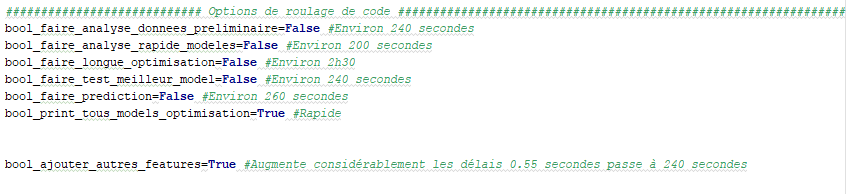
\includegraphics[width=\linewidth,height=6cm]{images/list_bool}

\begin{minted}[breaklines]{python}
############################ Options d'exécution du code ######################
bool_faire_analyse_donnees_preliminaire = True  # Environ 240 secondes
bool_faire_analyse_rapide_modeles = True  # Environ 200 secondes
bool_faire_longue_optimisation = True  # Environ 2h30
bool_faire_test_meilleur_model = True  # Environ 240 secondes
bool_faire_prediction = True  # Environ 260 secondes
bool_print_tous_models_optimisation = True  # Rapide
bool_ajouter_autres_features = True  # Augmente considérablement les délais .55 secondes passe à 240 secondes
\end{minted}

%\lstinputlisting[caption=Options d'exécution du code, style=customc]{exec.c}

\verb|bool_faire_analyse_donnees_preliminaire = True| permet de faire l'analyse préliminaire des données présentée dans la section \nameref{sec:analyse_prelim}. 

\verb|bool_faire_analyse_rapide_modeles = True| permet de faire l'analyse présentée dans la sous-section \nameref{subsec:modeles}. 

\verb|bool_faire_longue_optimisation = True| permet de compléter l'optimisation présentée dans la sous section \nameref{subsec:modeles}. 

\verb|bool_faire_test_meilleur_model = True| permet d'obtenir les résultats présentés dans la sous-section \nameref{subsec:simulation}. 

\verb|bool_faire_prediction = True| permet de faire les prédictions présentées dans la sous-section \nameref{subsec:predictions}. 

\verb|bool_print_tous_models_optimisation = True| permet d'afficher tous les résultats possibles de modèles créés dans la sous-section \nameref{subsec:optimisation}.

\verb|bool_ajouter_autres_features = True| permet de transformer les \emph{emojis} en texte et d'ajouter les attributs supplémentaires présentés à la section \nameref{sec:analyse_prelim}.